\documentclass[./../../paper.tex]{subfiles}
\graphicspath{{\subfix{./../../figures/}}}

\begin{document}


\autoref{fig:exp5-winner} displays the results of running each algorithm on a set of factuals. The figure shows clear dominance of the evolutionary model all the models across all datasets. 

\begin{figure}[htbp]
    \centering
    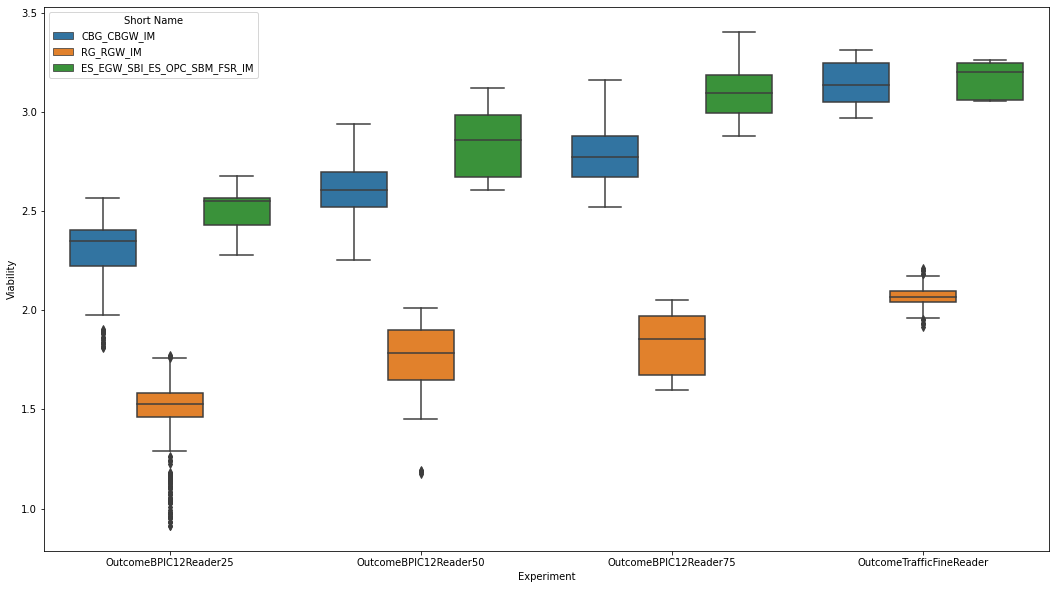
\includegraphics[width=\textwidth]{figures/generated/exp5_winner_overall.png}
    \caption{This figure shows boxplots of the viability of each models' generated counterfactuals across a herterogeneous set of datasets.}
    \label{fig:exp5-winner}
\end{figure}

Here, \optional{CBI-ES-UC3-SBM-RR } and \optional{CBI-RWS-OPC-SBM-FSR} display a higher median of viability across all datasets. This is surprising as the datasets are vastly different in sequence length and structure. The highest median is reached for \optional{CBI-ES-UC3-SBM-RR}

% TODO
% A notable observation occurs in the processing time. Although all models require more time to produce their results, if we increase the maximum length of sequences, the evolutionary algorithms require substiantially more time. \autoref{tbl:exp5_duration} shows, the processing time is much higher than the baseline models. On average, \attention{evo model} require \attention{duration in seconds}, while \attention{other models} require \attention{XX}, \attention{XX} and \attention{XX}, respectively.


\end{document}